%% Copyright 2007-2020 Elsevier Ltd
%% 
%% This file is part of the 'Elsarticle Bundle'.
%% ---------------------------------------------
%% 
%% It may be distributed under the conditions of the LaTeX Project Public
%% License, either version 1.2 of this license or (at your option) any
%% later version.  The latest version of this license is in
%%    http://www.latex-project.org/lppl.txt
%% and version 1.2 or later is part of all distributions of LaTeX
%% version 1999/12/01 or later.
%% 
%% The list of all files belonging to the 'Elsarticle Bundle' is
%% given in the file `manifest.txt'.
%% 
%% Template article for Elsevier's document class `elsarticle'
%% with harvard style bibliographic references

\documentclass[review,12pt,authoryear]{elsarticle}

%% Use the option review to obtain double line spacing
%% \documentclass[authoryear,preprint,review,12pt]{elsarticle}

%% Use the options 1p,twocolumn; 3p; 3p,twocolumn; 5p; or 5p,twocolumn
%% for a journal layout:
%% \documentclass[final,1p,times,authoryear]{elsarticle}
%% \documentclass[final,1p,times,twocolumn,authoryear]{elsarticle}
%% \documentclass[final,3p,times,authoryear]{elsarticle}
%% \documentclass[final,3p,times,twocolumn,authoryear]{elsarticle}
%% \documentclass[final,5p,times,authoryear]{elsarticle}
%% \documentclass[final,5p,times,twocolumn,authoryear]{elsarticle}

%% For including figures, graphicx.sty has been loaded in
%% elsarticle.cls. If you prefer to use the old commands
%% please give \usepackage{epsfig}

%% The amssymb package provides various useful mathematical symbols
\usepackage{amssymb}
%% The amsthm package provides extended theorem environments
%% \usepackage{amsthm}

%% The lineno packages adds line numbers. Start line numbering with
%% \begin{linenumbers}, end it with \end{linenumbers}. Or switch it on
%% for the whole article with \linenumbers.
\usepackage{lineno}

% for adjusting table width automatically
\usepackage{adjustbox}
\usepackage{tabulary, ragged2e}
\usepackage{booktabs}
\usepackage{multirow}
\usepackage{csvsimple}
\usepackage{longtable}
\journal{Geography and Sustainability}

\begin{document}
\begin{frontmatter}

\title{The influence of resource use on yield versus sale price trade-off in Australian vineyards}

\affiliation[label1]{organization={Queensland University of Technology}}
\affiliation[label2]{organization={Australian Wine Research Institute}}
\affiliation[label3]{organization={Food Agility CRC}}
 \author[label1,label2,label3]{Bryce Boyd}
 \author[label1]{Kate Helmstedt}
 \author[label2]{Mardi Longbottom}
 \author[label1]{Kerrie Mengersen}

 \begin{highlights}
    \item Comparative analysis of resource use, average sale price and quantity in Australian winegrowing.
    \item Regional comparison of outcomes and resource use in Australian winegrowing regions.
    \item Baseline models for comparing vineyards.
    \item Analysis of national, decade long data source.
  \end{highlights}

 \begin{abstract}
    % The word limit needs to be checked.
    When strategies for a sustainable winegrowing industry are assessed, there is a trade-off between balancing the amount of resources invested and the resultant yield and sale price of the produce. In this analysis we observe relationships between resource use, yield and sale price through the use of statistical models. The dataset used for this analysis includes data collected for the past 10 years from 1261 vineyards located over a diverse range of Australian winegrowing regions. Yield and sale price were evaluated with respect to the resource use factors water use and Green House Gas (GHG) emissions. The analysis confirmed a strong relationship between area and resource use, with the overall area of a vineyard and its access to resources greatly determining the upper limit of yield. However, area was also negatively related to the average sale price of grapes; we find that higher average sale prices were connected to high resource inputs per area, rather than to the overall expenditure of resources. Regional and temporal effects on vineyard yield and average sales price were also identified. Overall, the analysis highlighted the importance of considering a vineyard's business goal, region, external pressures and economies of scale, when considering whether to pursue higher yields or higher average sales prices.
    \end{abstract}
    %%Graphical abstract`
    %\begin{graphicalabstract}
     % 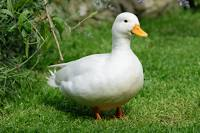
\includegraphics{graphical_abstract.jpeg}
    %\end{graphicalabstract}'
    
    %\begin{keyword}
    %% keywords here, in the form: keyword \sep keyword
    %Keyword one \sep{} keyword two
    %% PACS codes here, in the form: \PACS code \sep code
    %\PACS{} 0000 \sep{} 1111
    %% MSC codes here, in the form: \MSC code \sep code
    %% or \MSC[2008] code \sep code (2000 is the default)
    %\MSC{} 0000 \sep{} 1111
    %\end{keyword}
    %%Research highlights

\end{frontmatter}
\end{document}